%%%%%%%%%%%%%%%%%%%%%%%%%%%%%%%%%%%%%%%%%%%%%%%%%%%%%%%%%%%%%%%%%%%%%%%%%%%%%%%%%%%%%%%%%%%%%%%%%%%%%%
%
%   Filename    : appendix_A.tex 
%
%   Description : This file is for including the Research Ethics Documents (delegated as Appendix A) 
%                 
%%%%%%%%%%%%%%%%%%%%%%%%%%%%%%%%%%%%%%%%%%%%%%%%%%%%%%%%%%%%%%%%%%%%%%%%%%%%%%%%%%%%%%%%%%%%%%%%%%%%%%

\chapter{Data Gathering Documentation and Supplementary Analysis}
\label{sec:appendixa}



% Save the file you want to include in PDF format.
% Uncomment the commant below specifying the correct appendix file. 
%\includepdf[pages=-, scale = 0.9, pagecommand={}, offset = -30 0]{appendixA.pdf}

\begin{figure}[!htbp]
	\centering
	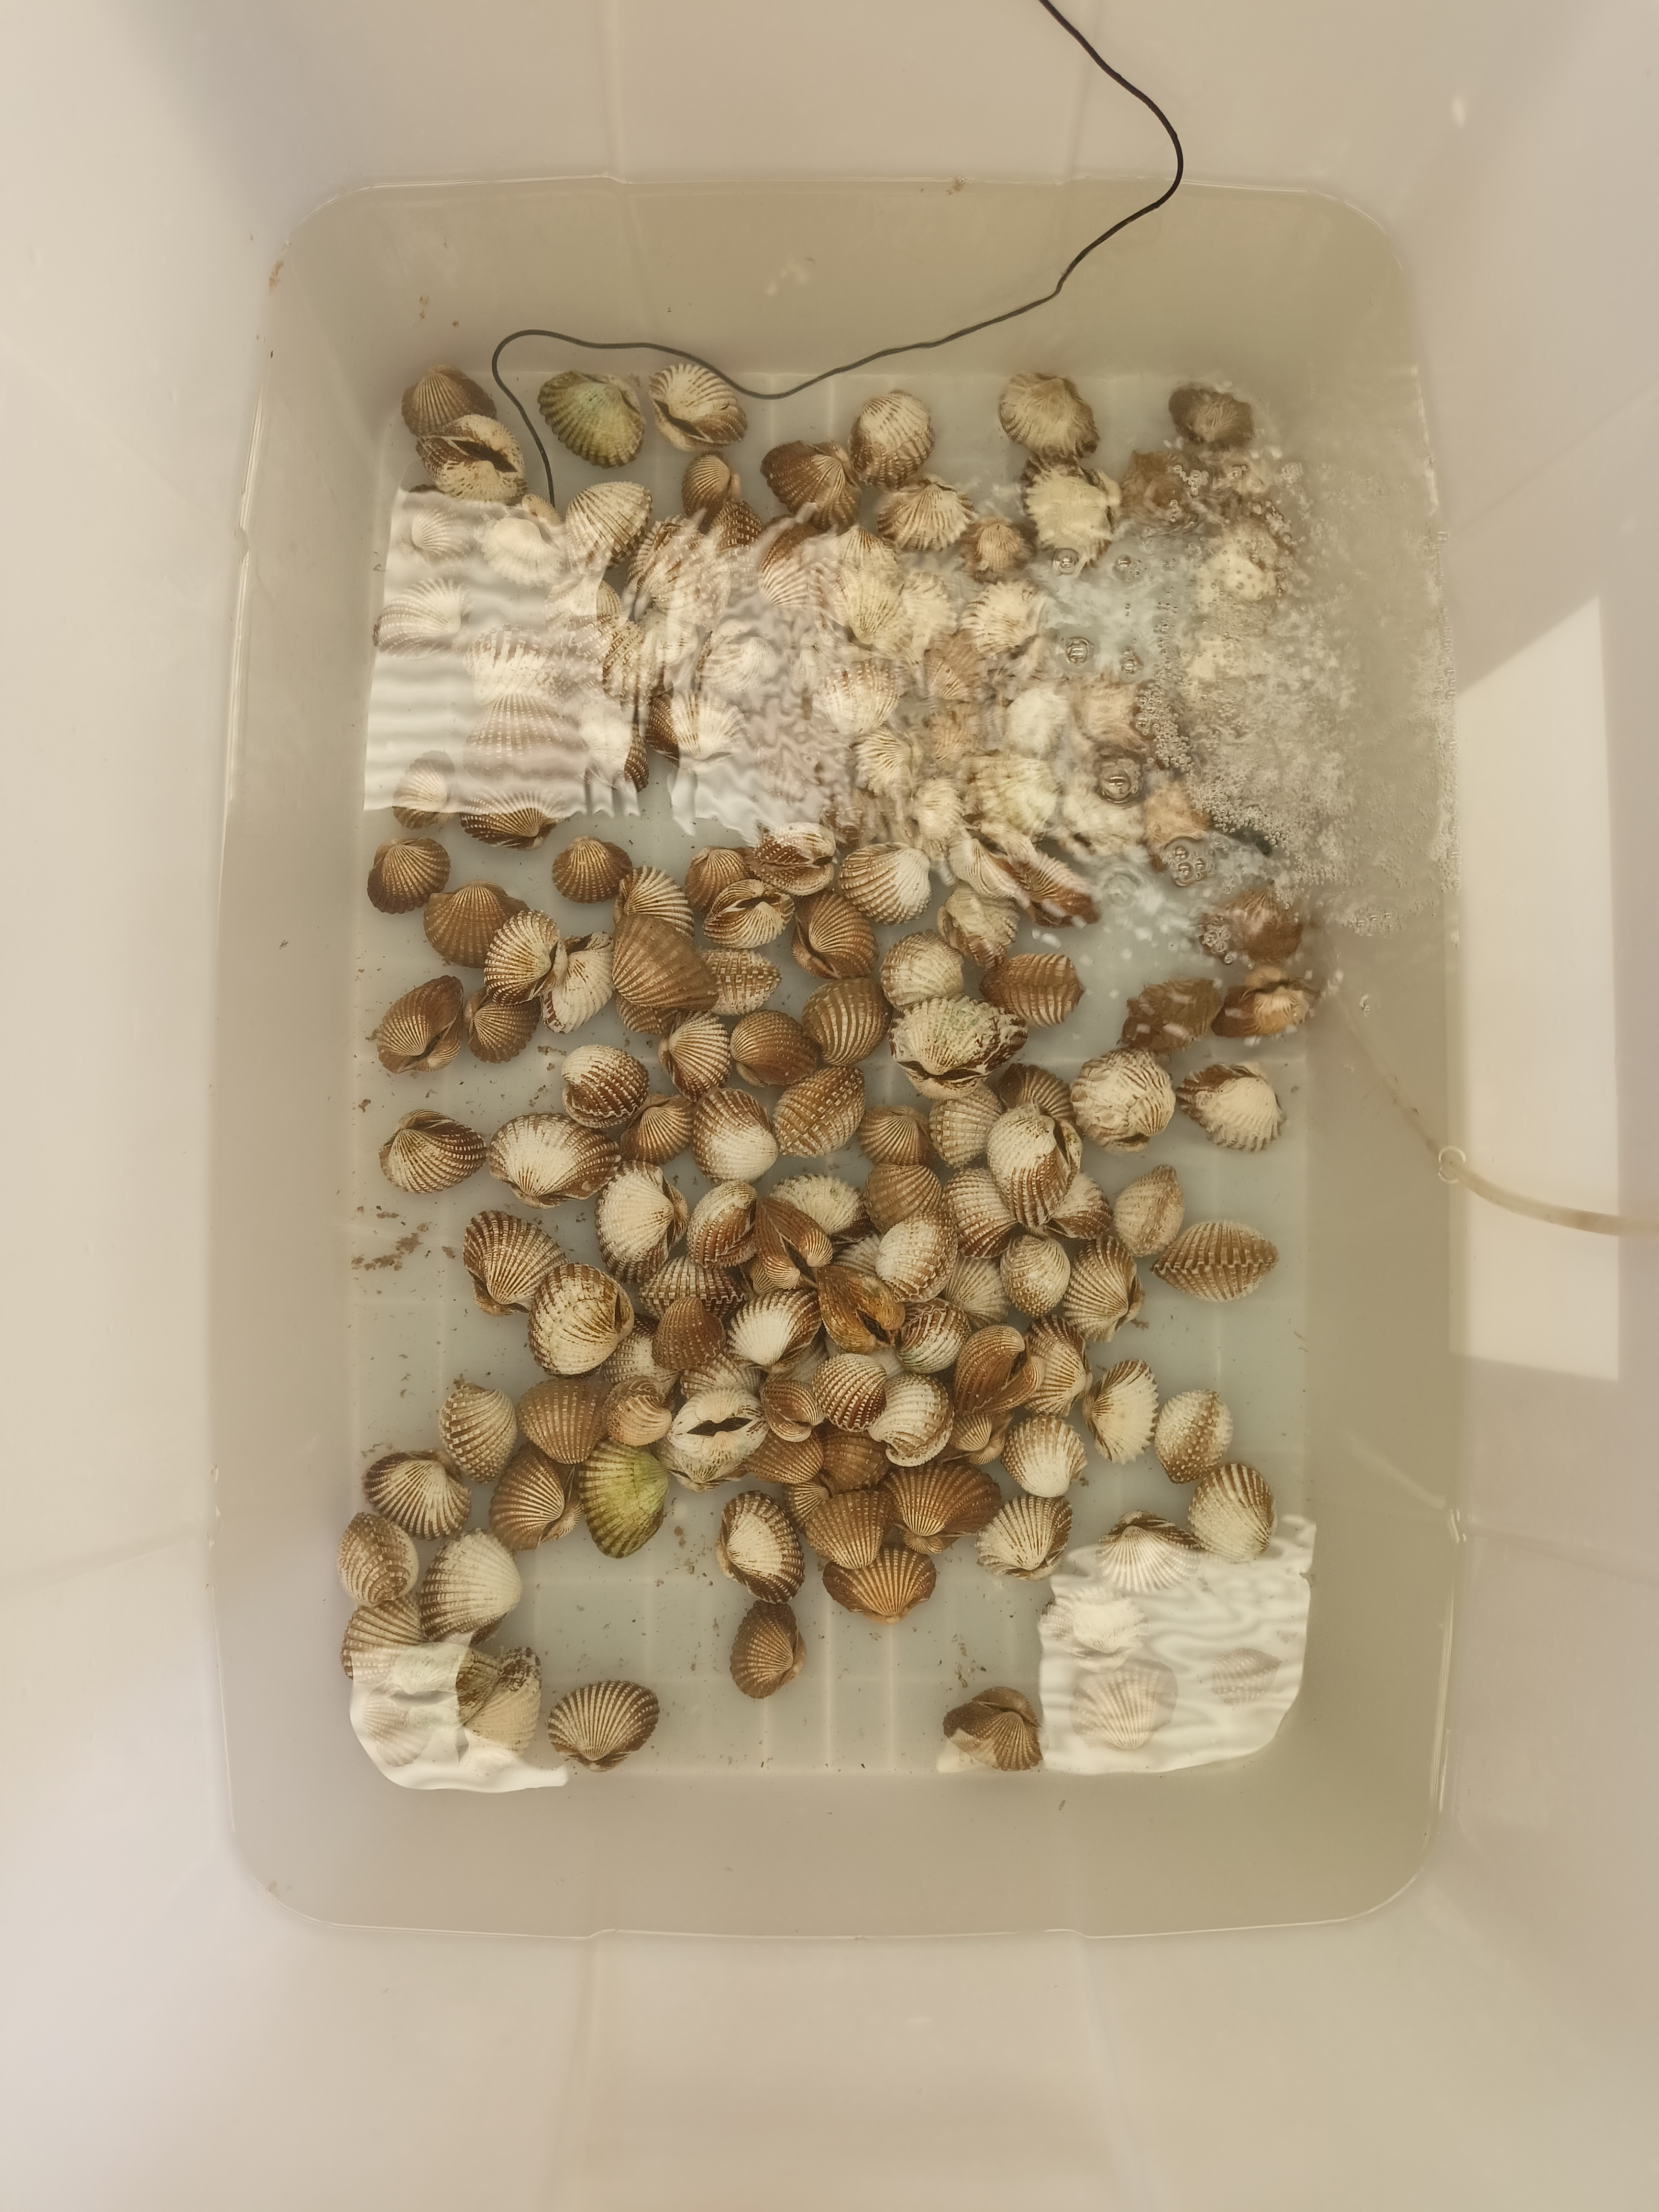
\includegraphics[width=0.4\textwidth, angle=90]{figures/spawning.jpg}
	\caption{Sex Identification Through Spawning of \Tegillarcagranosa}
\end{figure}

\begin{figure}[!htbp]
	\centering
	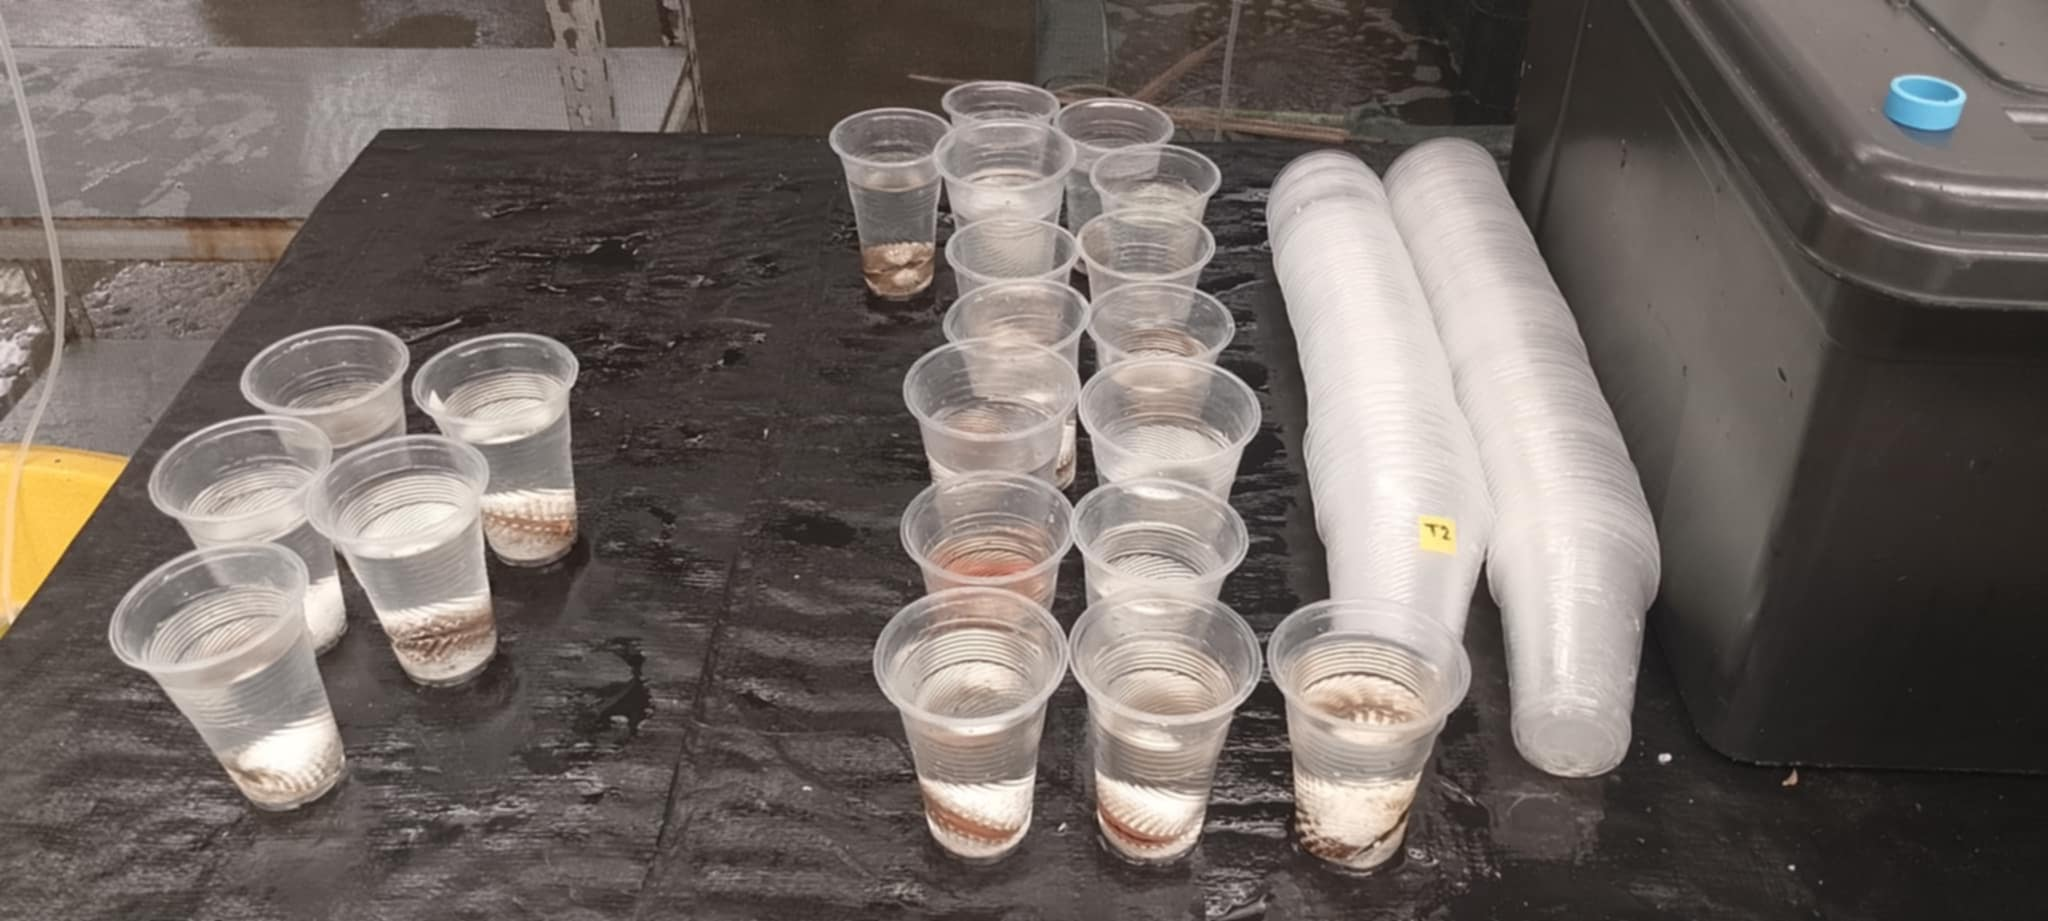
\includegraphics[width=0.6\textwidth]{figures/spawning_separated.jpg}
	\caption{Separating Male and Female Samples After Spawning of \Tegillarcagranosa}
\end{figure}

\begin{figure}[!htbp]
	\centering
	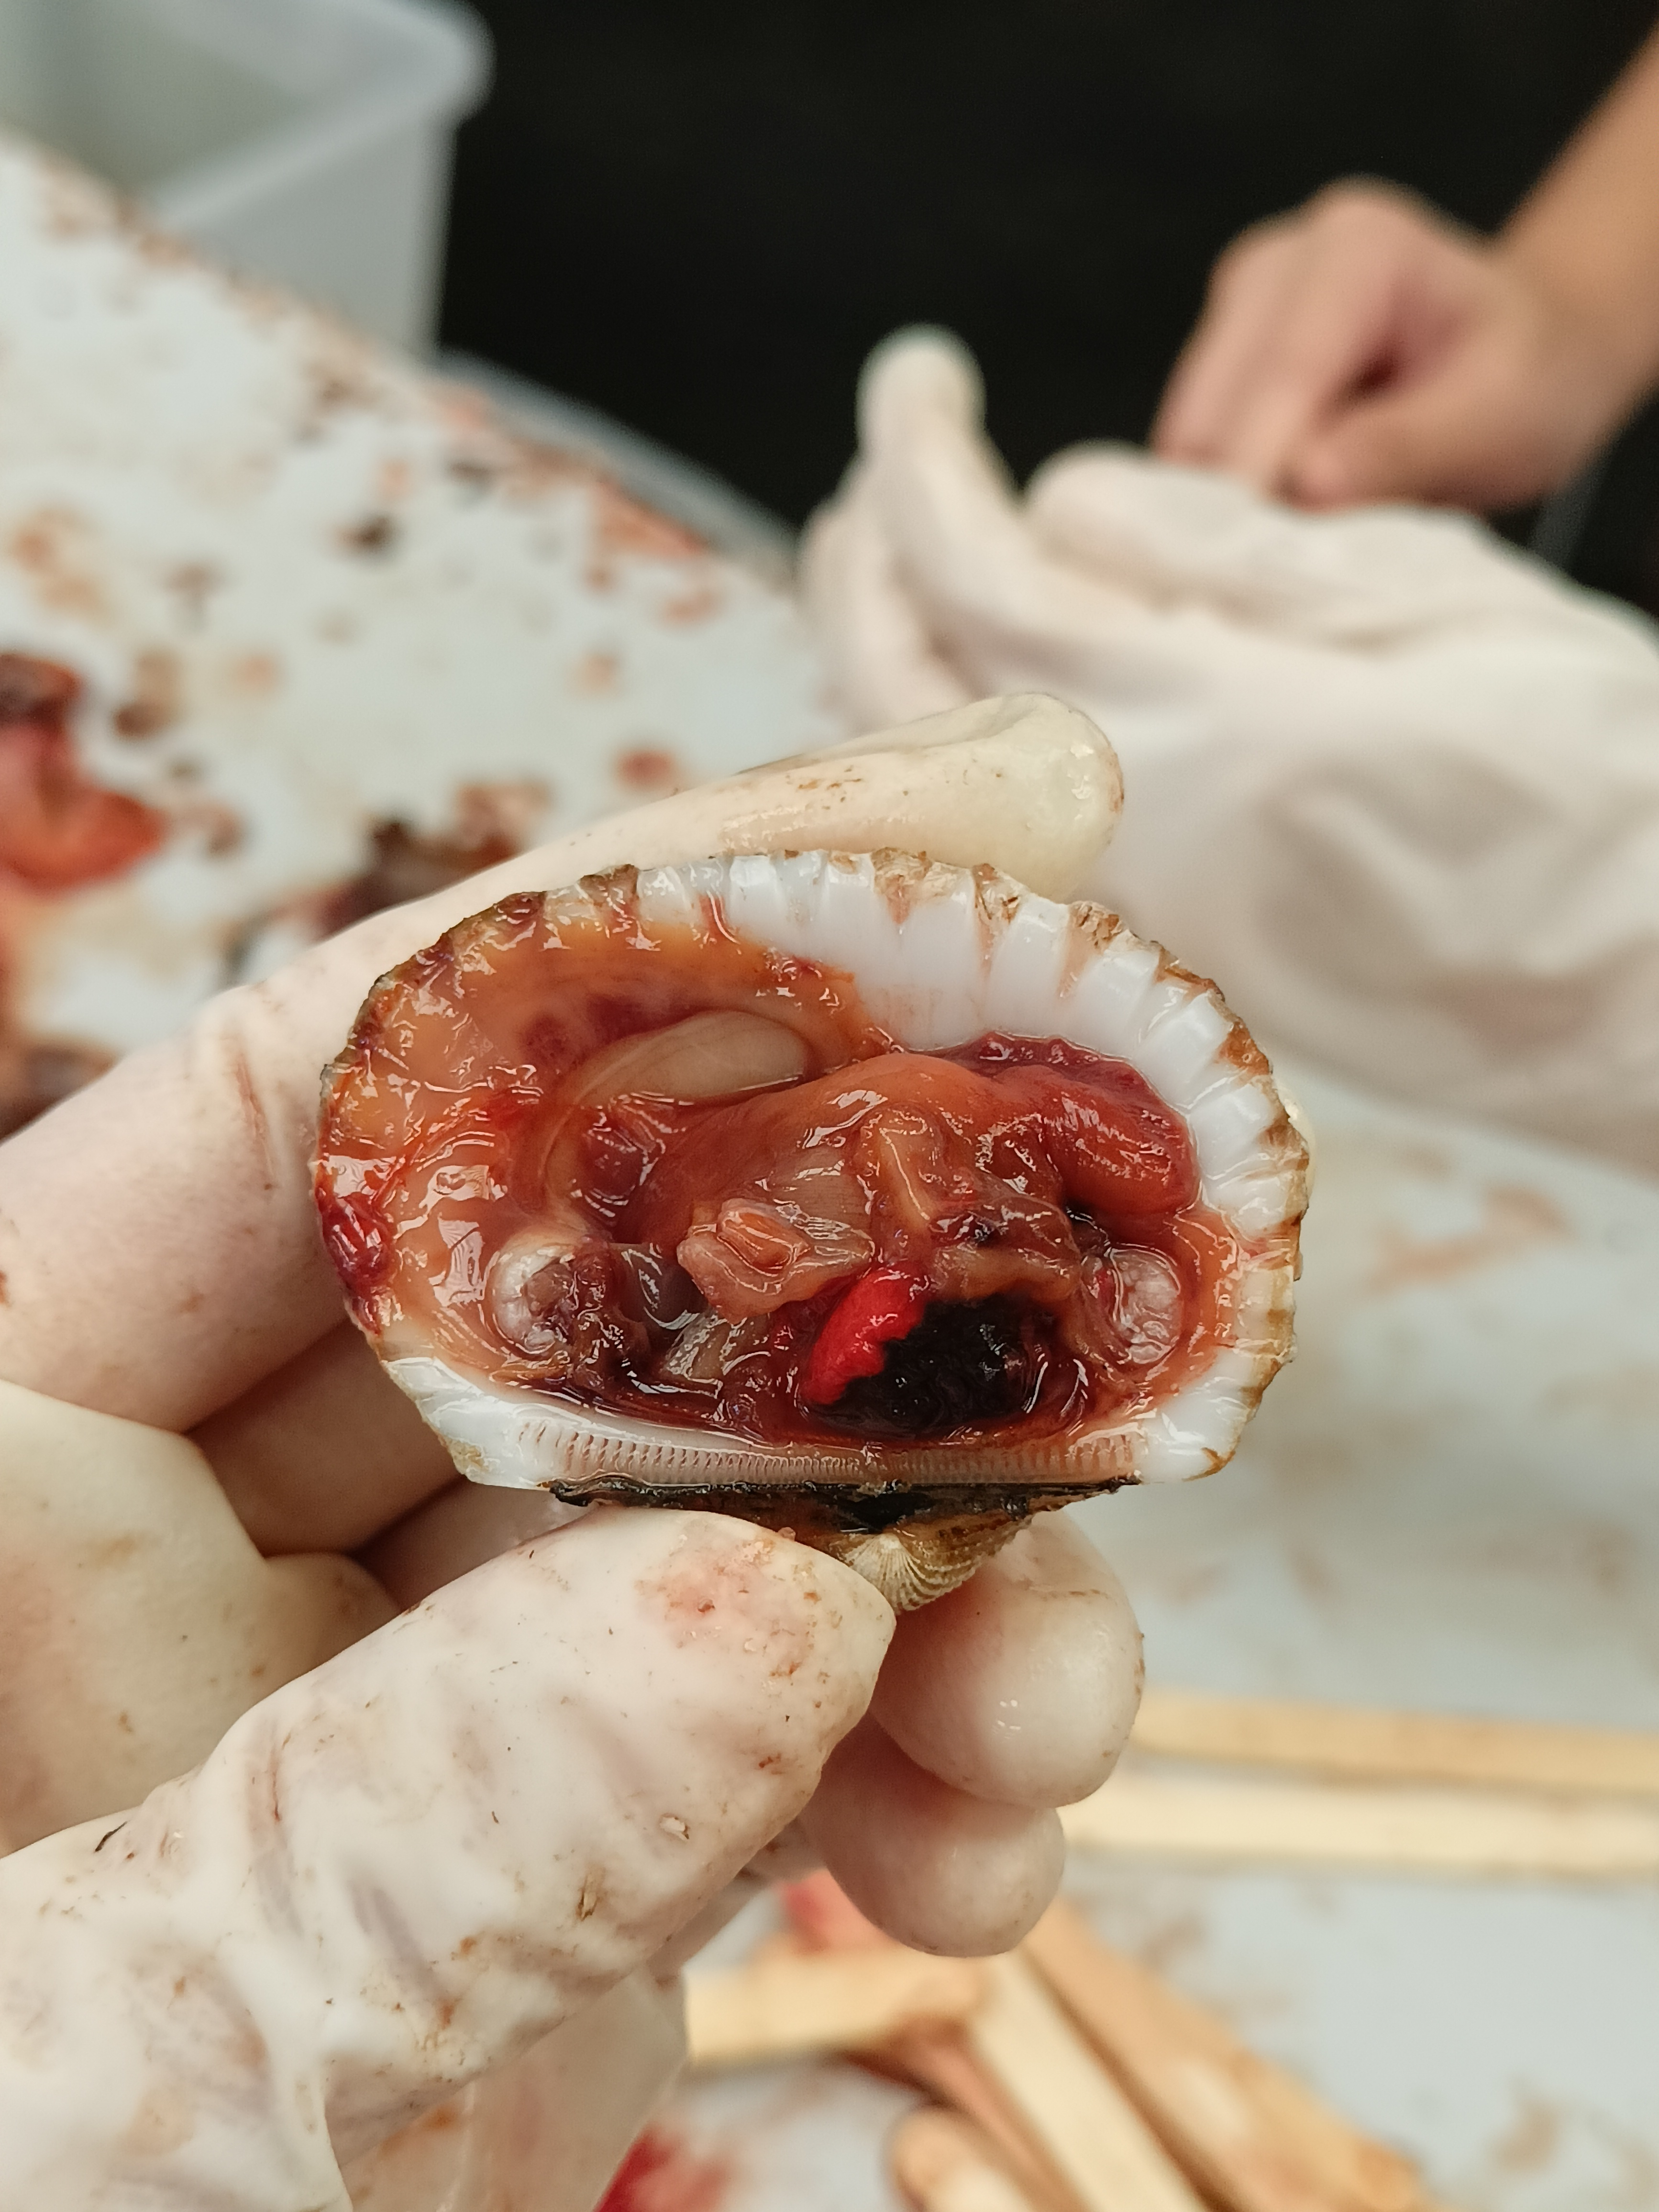
\includegraphics[width=0.4\textwidth, angle=90]{figures/dissecting_female.jpg}
	\caption{Sex Identified Female Through Dissecting of \Tegillarcagranosa}
\end{figure}

\begin{figure}[!htbp]
	\centering
	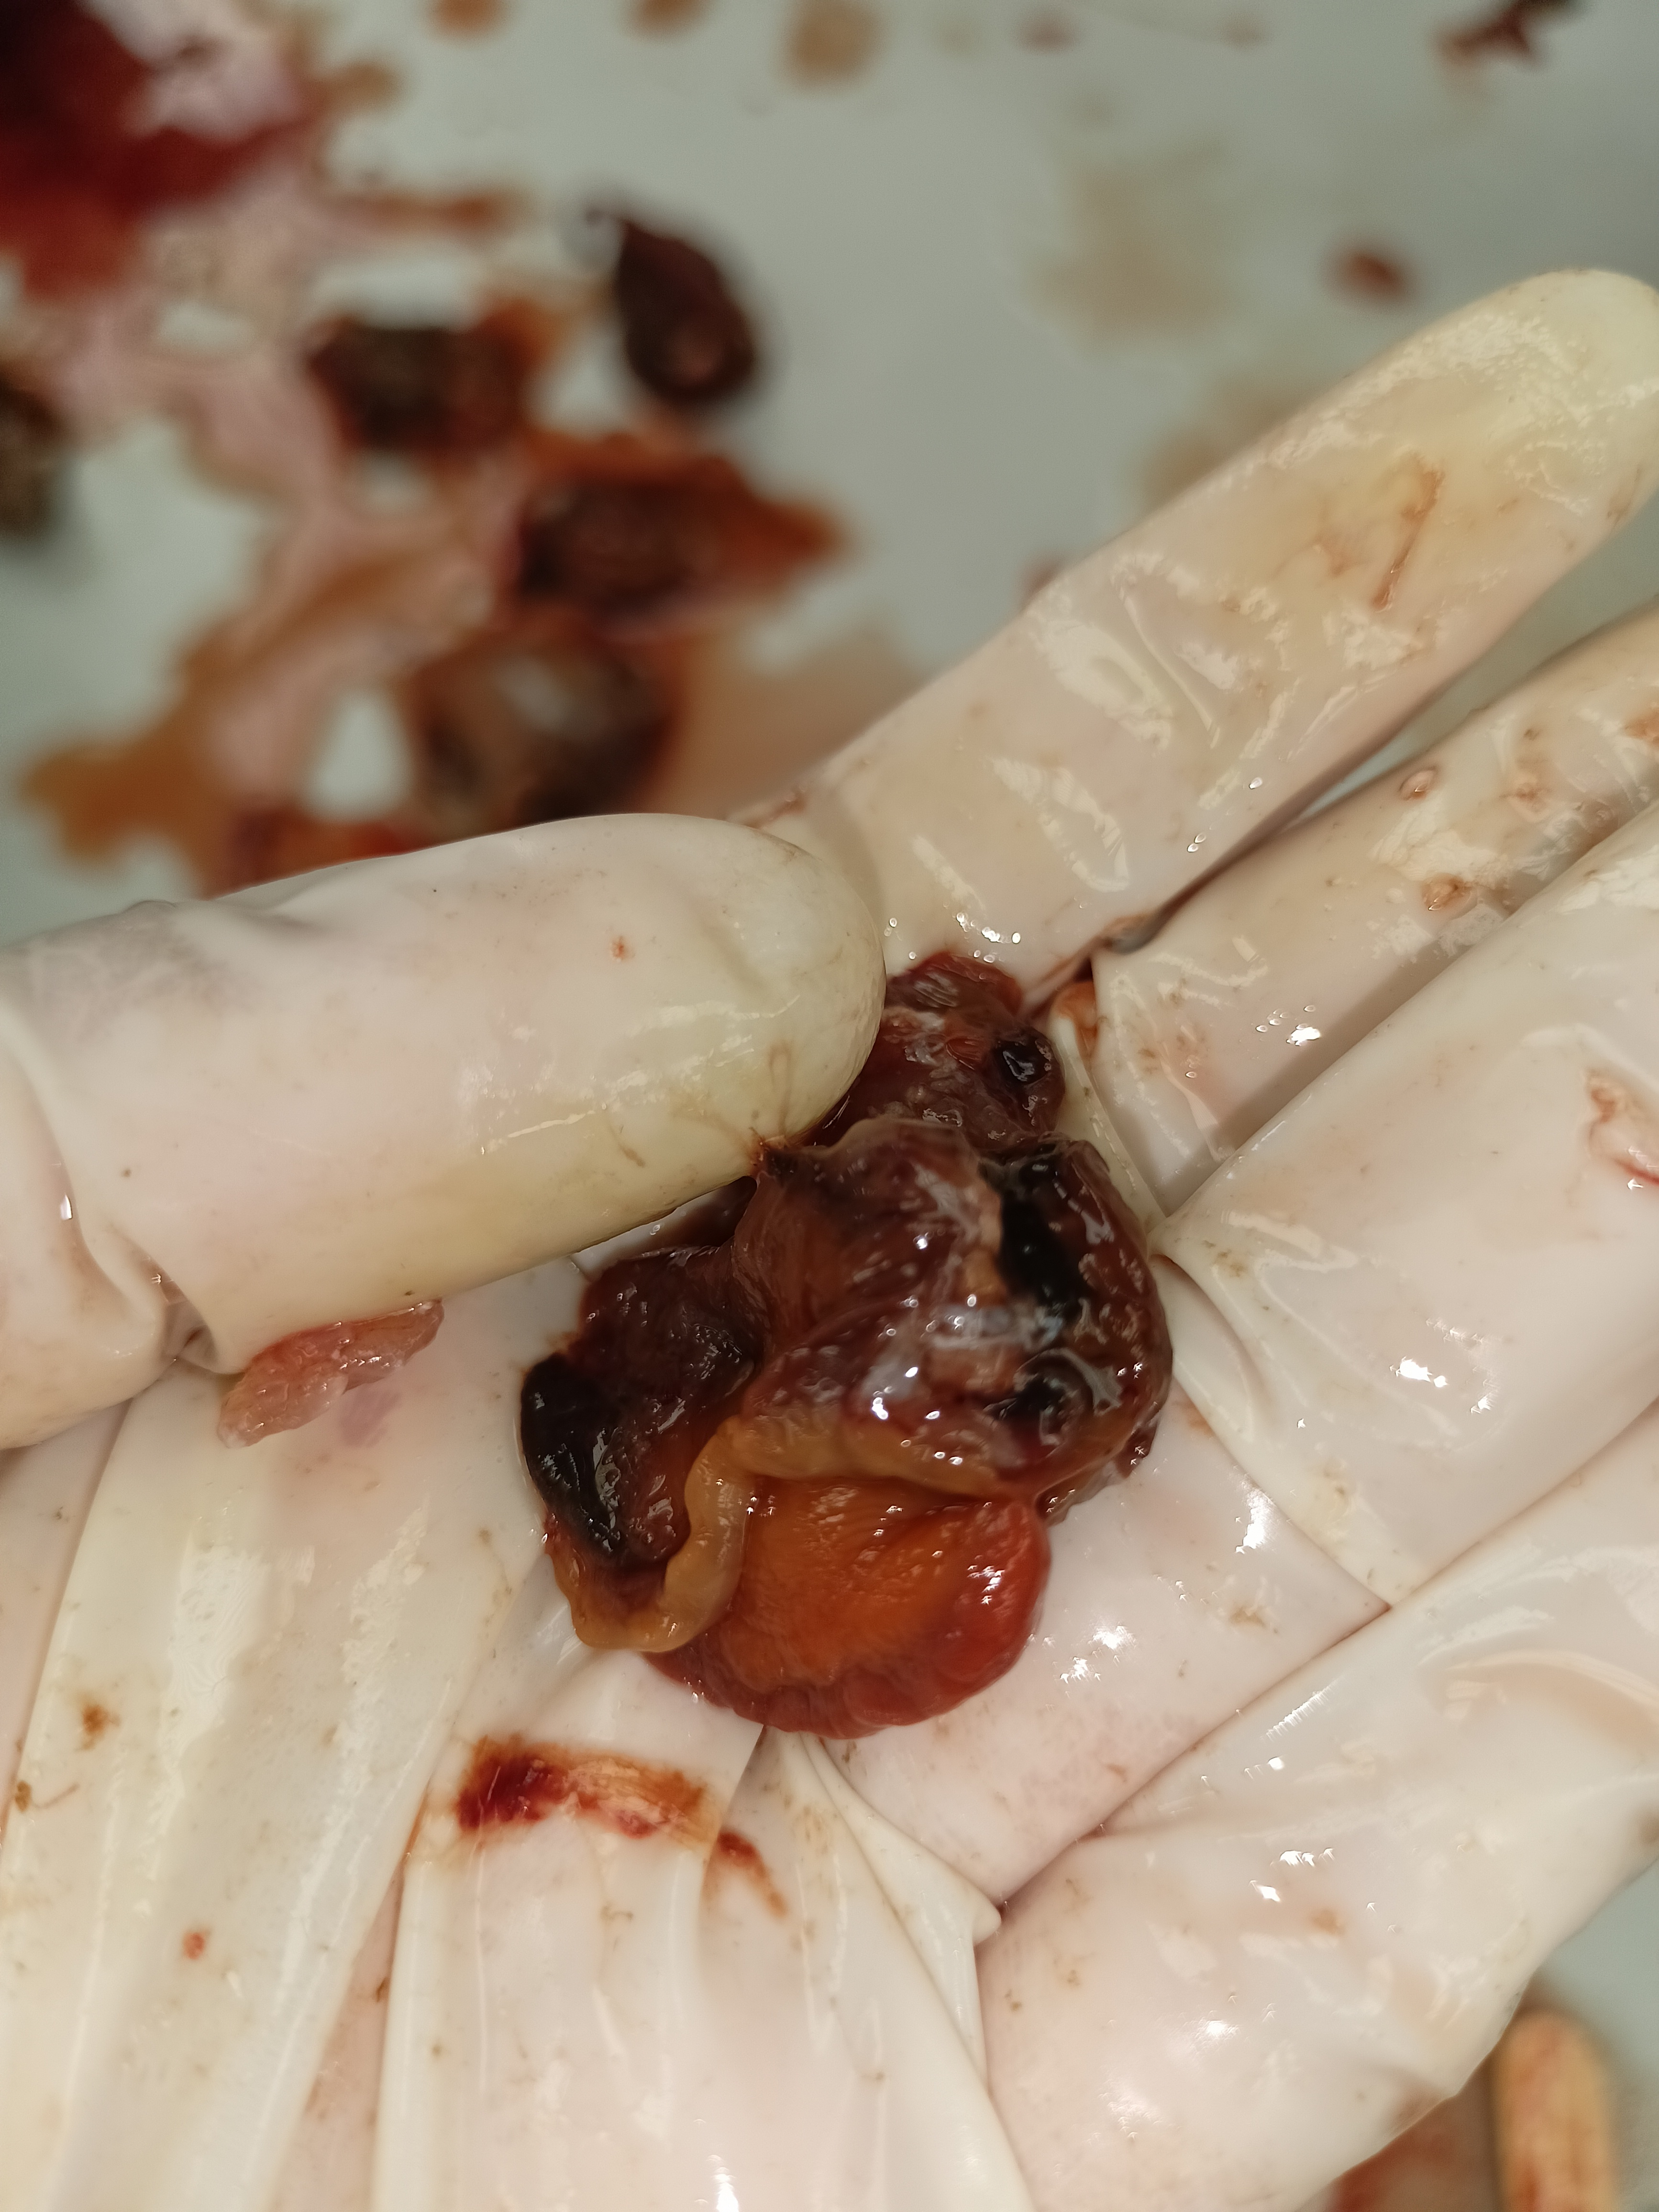
\includegraphics[width=0.4\textwidth, angle=90]{figures/dissecting male.jpg}
	\caption{Sex Identified Male Through Dissecting of \Tegillarcagranosa}
\end{figure}

\begin{figure}[!htbp]
	\centering
	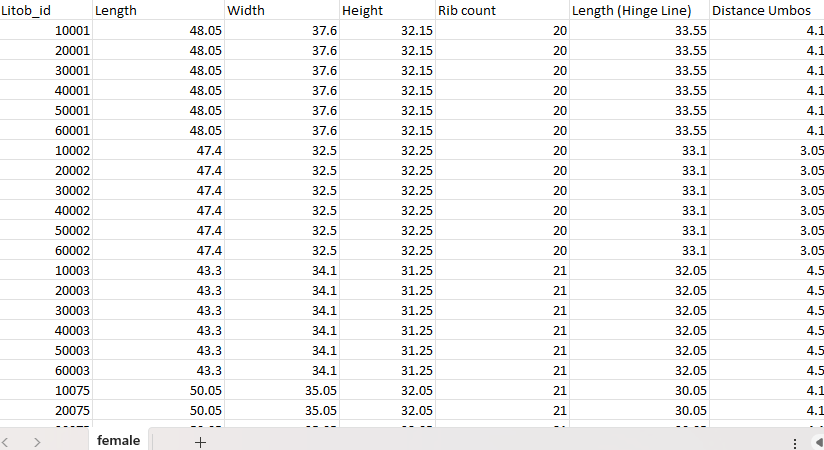
\includegraphics[width=0.6\textwidth]{figures/female_dataset.png}
	\caption{Linear Measurements of Female \Tegillarcagranosa}
\end{figure}

\begin{figure}[!htbp]
	\centering
	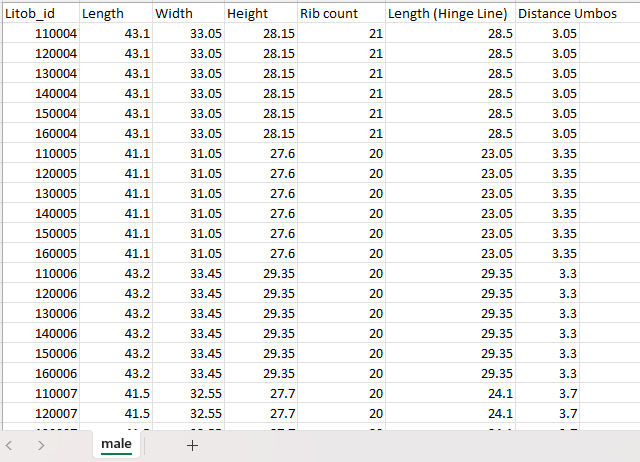
\includegraphics[width=0.6\textwidth]{figures/male_dataset.png}
	\caption{Linear Measurements of Male \Tegillarcagranosa}
\end{figure}

\begin{figure}[!htbp]
	\centering
	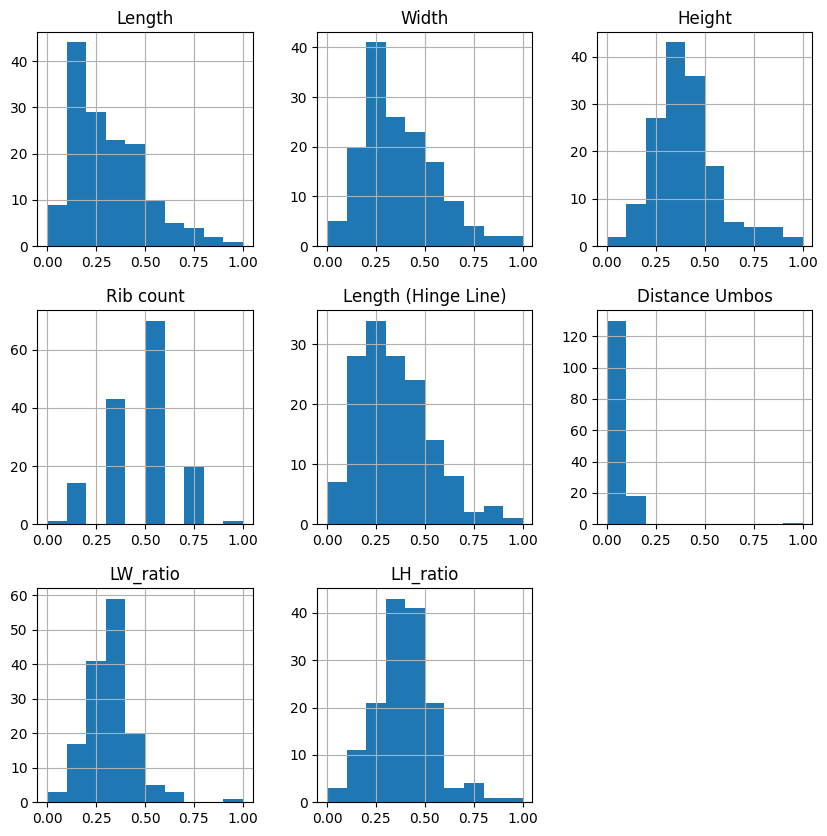
\includegraphics[width=0.6\textwidth]{figures/sample_distribution.png}
	\caption{Distribution of the Features of \Tegillarcagranosa}
\end{figure}


